% Chapter where we present the results.

\chapter{Results}
\label{ch:results}

In Chapter \ref{ch:methods}, we discussed a general solution to the automatic
protoboard
layout problem and various alternatives that can be used in implementing the
solution. Figure \ref{fig:alternatives} summarizes the alternatives.
In this chapter, we provide quantitative data comparing the alternative
strategies, and the data is discussed in Chapter \ref{ch:discussion}.

\begin{figure}[H]
\centering
\subfigure{
\Tree [{Distance} {Blocking} {Random} ].Placement
}
\subfigure{
\Tree [{All pairs}
       [Increasing Decreasing ].{Per-node}
       [Increasing Decreasing ].{Per-pair}
       {Straight} ].Wiring
}\\
\subfigure{
\Tree [{$A*$} {Best First} ].Search
}
\caption[Algorithm alternatives summary]{Summary of possible alternatives
to the algorithm.}
\label{fig:alternatives}
\end{figure}

As comparing all $3 \times 6 \times 2 = 36$ possible implementations of the
algorithm is tedious,
we analyzed the three different means for alternatives (placement, wiring, and
search) separately. We carried out the following comparisons:

\begin{enumerate}
\item Placement: Blocking vs. Distance vs. Random. The wiring method was per-pair
(decreasing), and we used $A*$ Search.
\item Wiring: All pairs vs. Per-node (increasing) vs. Per-node (decreasing) vs.
Per-pair (increasing) vs. Per-pair (decreasing) vs. Straight.
The placement method was blocking, and we used $A*$ Search.
\item Search: $A*$ vs. Best First. The placement method was blocking, and the
wiring method was per-pair (decreasing).
\end{enumerate}

The data to compare the alternatives were gathered as described in Chapter
\ref{ch:methods}. We ran the algorithm on $4425$ randomly generated schematics
of varying complexities. The algorithm was run $10$ times on each schematic.

In comparing alternatives, we consider $3$ questions:
\begin{enumerate}
\item Which alternative is successful most often?
\item Which alternative, when successful, takes the least amount of time?
\item Which alternative, when successful, produces the best layouts?
\end{enumerate}

We are also interested in how each of these attributes (success rate, running
time, and layout quality) varies with circuit complexity. To quantify
the complexity of a circuit, we look at the number of pins in the
circuit, where a pin is defined to be a connection point on a circuit
component that is connected by wires to another connection point (on the same
component or a different component). Figure
\ref{fig:complexity_hist} presents a histogram of the number of pins in the
schematics that were used to do all comparisons in this chapter,
not including the data presented in Section \ref{sec:combined_algorithm}, for
which we used a newly generated dataset of schematics to analyze the performance
of the combined algorithm. Note that there are fewer samples of schematics
of the lowest and highest circuit complexities. Hence, the statistics given
for the extreme complexities are less informative.

\begin{figure}[H]
\begin{center}
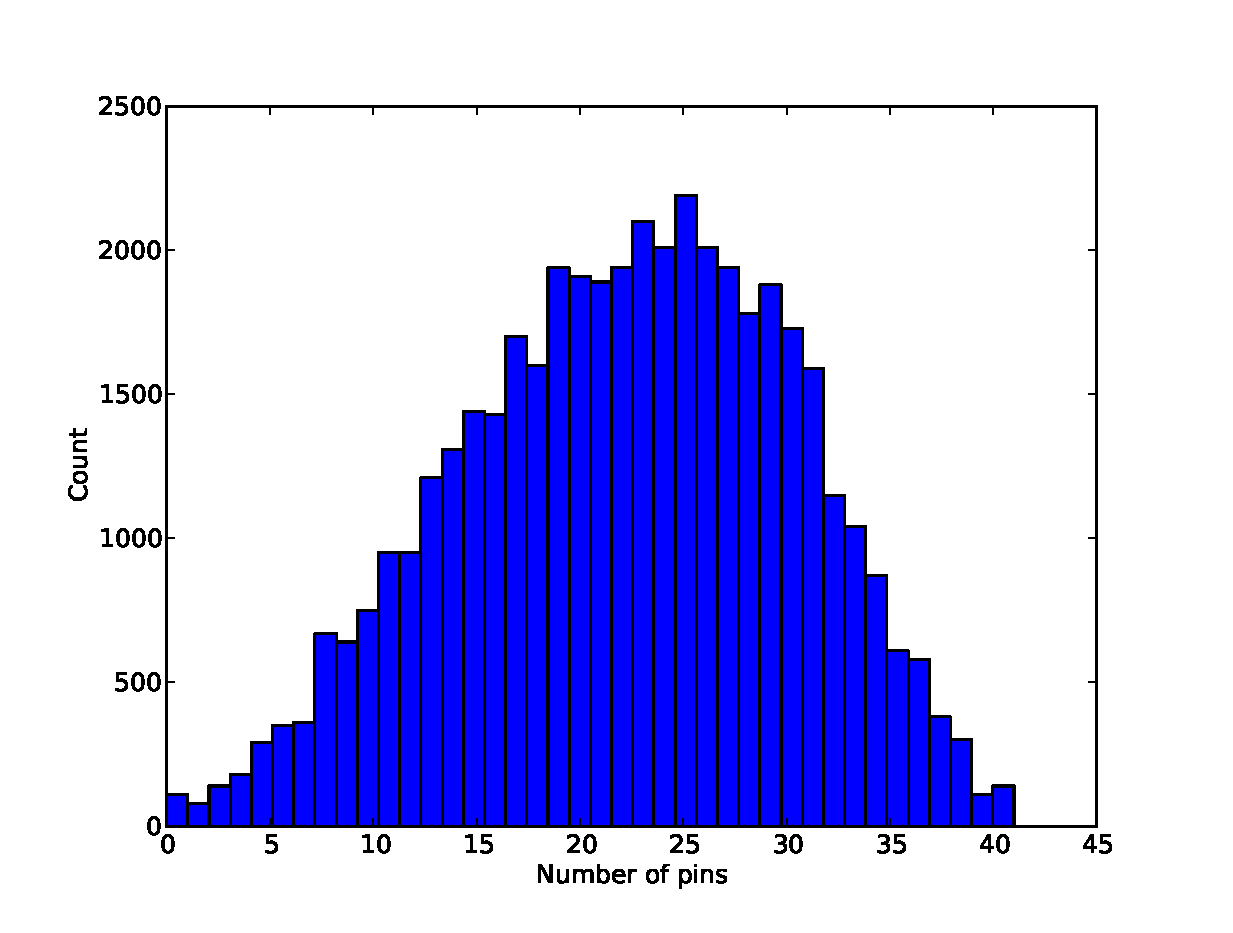
\includegraphics[width=\textwidth]{Images/complexity_hist.eps}
\caption[Schematic complexity histogram]{Histogram of the complexities, in terms
of numbers of pins, of the $4425$ schematics used for evaluation.}
\label{fig:complexity_hist}
\end{center}
\end{figure}

To compare success rates, we look at number of successes out of $10$ runs
on each of the $4425$ schematics. To compare running time, we look at CPU
time spent on the wiring step, as the placement step has much less variability.
To compare the goodness of layouts, we look at numbers of wires, total
lengths of wires, numbers of wire crosses, and our layout badness metric as
functions of circuit complexity. Note that in all figures that follow,
error bars indicate $1.96$ times the standard error. For each comparison,
we present exemplar layouts generated by the alternative methods for the
schematic shown in Figure \ref{fig:exemplar_schematic}.

\begin{figure}
\begin{center}
\includegraphics[width=\textwidth]{Images/exemplar_schematic.png}
\caption[Exemplar schematic]{Schematic used to generate the exemplar protoboard
layouts.}
\label{fig:exemplar_schematic}
\end{center}
\end{figure}

\section{Random Layout}
\label{sec:random_layout}

Before embarking upon the comparisons, we give an exemplar of a protoboard
layout generated completely at random. Here, we choose an op-amp packaging
randomly, and we place each circuit piece randomly,
only taking care not to place two pieces that share a $5$-column, and
not obeying any other restrictions. This method of random placement, is,
therefore, different from the one described in Section
\ref{sec:random_placement}. We then use Straight wiring. Figure
\ref{fig:completely_random} presents a layout generated for the schematic
shown in Figure \ref{fig:exemplar_schematic}. This completely random layout
method is compared against the final algorithm in Section
\ref{sec:combined_algorithm}.

\begin{figure}[H]
\begin{center}
\includegraphics[width=\textwidth]{Images/exemplar_completely_random.png}
\caption[Random layout exemplar]{Exemplar for the completely random method.}
\label{fig:completely_random}
\end{center}
\end{figure}

\section{Comparing Placement Methods}
\label{sec:compare_placement}

\begin{figure}[H]
\begin{center}
\includegraphics[width=\textwidth]{Images/exemplar_per_pair_decreasing.png}
\caption[Blocking placement method exemplar]{Exemplar for the blocking placement
method, using per-pair (decreasing) wiring and $A*$ Search.}
\end{center}
\end{figure}

\begin{figure}[H]
\begin{center}
\includegraphics[width=\textwidth]{Images/exemplar_distance.png}
\caption[Distance placement method exemplar]{Exemplar for the distance placement
method,
using per-pair (decreasing) wiring and $A*$ Search.}
\end{center}
\end{figure}

\begin{figure}[H]
\begin{center}
\includegraphics[width=\textwidth]{Images/exemplar_random_placement.png}
\caption[Random placement method exemplar]{Exemplar for the random placement
method, using per-pair (decreasing) wiring and
$A*$ Search. As the random
placement method performs too poorly to generate layouts for complex circuits,
this exemplar was
generated for the schematic shown in Figure \ref{fig:gui_example}.
For comparison, another layout for the same schematic is given in Figure
\ref{fig:cmax_sample}.}
\end{center}
\end{figure}

\begin{figure}[H]
\begin{center}
\includegraphics[width=\textwidth]{Images/placement_success_comparison.eps}
\caption[Placement method success rate comparison]{Placement method success rate
comparison.}
\label{fig:placement_success}
\end{center}
\end{figure}

\begin{table}[H]
\begin{center}
\begin{singlespace}
\begin{tabular}{|c||c|c|c|c|c|c|c|c|c|c|c|}
\hline
 & \multicolumn{11}{|c|}{Number of times succeeded out of $10$} \\
\hline
 & 0 & 1 & 2 & 3 & 4 & 5 & 6 & 7 & 8 & 9 & 10 \\
\hline\hline
Blocking & $162$ & $38$ & $51$ & $57$ & $72$ & $85$ & $109$ & $106$ & $144$ & $203$ & $3398$ \\
 & $0.04$ & $0.01$ & $0.01$ & $0.01$ & $0.02$ & $0.02$ & $0.02$ & $0.02$ & $0.03$ & $0.05$ & $0.77$ \\
\hline
 Distance & $258$ & $55$ & $54$ & $50$ & $52$ & $77$ & $86$ & $97$ & $93$ & $130$ & $3473$ \\
  & $0.06$ & $0.01$ & $0.01$ & $0.01$ & $0.01$ & $0.02$ & $0.02$ & $0.02$ & $0.02$ & $0.03$ & $0.78$ \\
\hline
  Random & $893$ & $512$ & $387$ & $364$ & $292$ & $259$ & $247$ & $277$ & $311$ & $321$ & $562$ \\
   & $0.20$ & $0.12$ & $0.09$ & $0.08$ & $0.07$ & $0.06$ & $0.06$ & $0.06$ & $0.07$ & $0.07$ & $0.13$ \\
\hline
\end{tabular}
\end{singlespace}
\end{center}
\caption[Placement method success rate comparison]{This is an alternative
presentation of the data given in Figure \ref{fig:placement_success}. Each cell
in the table gives the count (and percentage out of the total $4425$)
of schematics for which a
particular method succeeded a given number times out of $10$ runs.}
\label{tb:placement_success}
\end{table}

\begin{figure}
\begin{center}
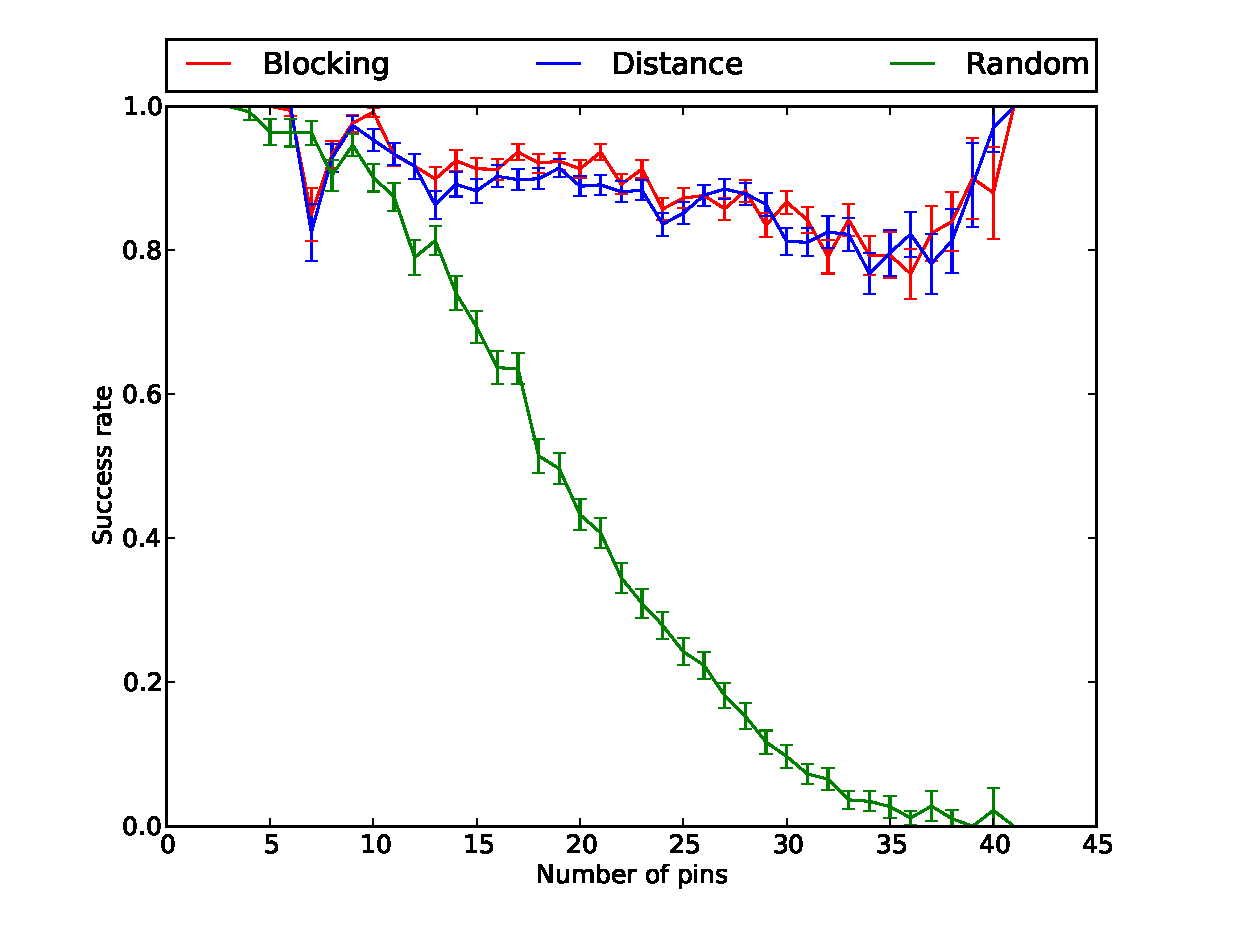
\includegraphics[width=\textwidth]{Images/placement_success_trend_comparison.eps}
\caption[Placement method success rate trend comparison]{Placement method
success rate trend comparison.}
\label{fig:placement_success_trend}
\end{center}
\end{figure}

\begin{figure}
\begin{center}
\includegraphics[width=\textwidth]{Images/placement_time_trend_comparison.eps}
\caption[Placement method wiring time trend comparison]{Placement method wiring
time trend comparison for successful runs.}
\label{fig:placement_time_trend}
\end{center}
\end{figure}

\begin{figure}
\begin{center}
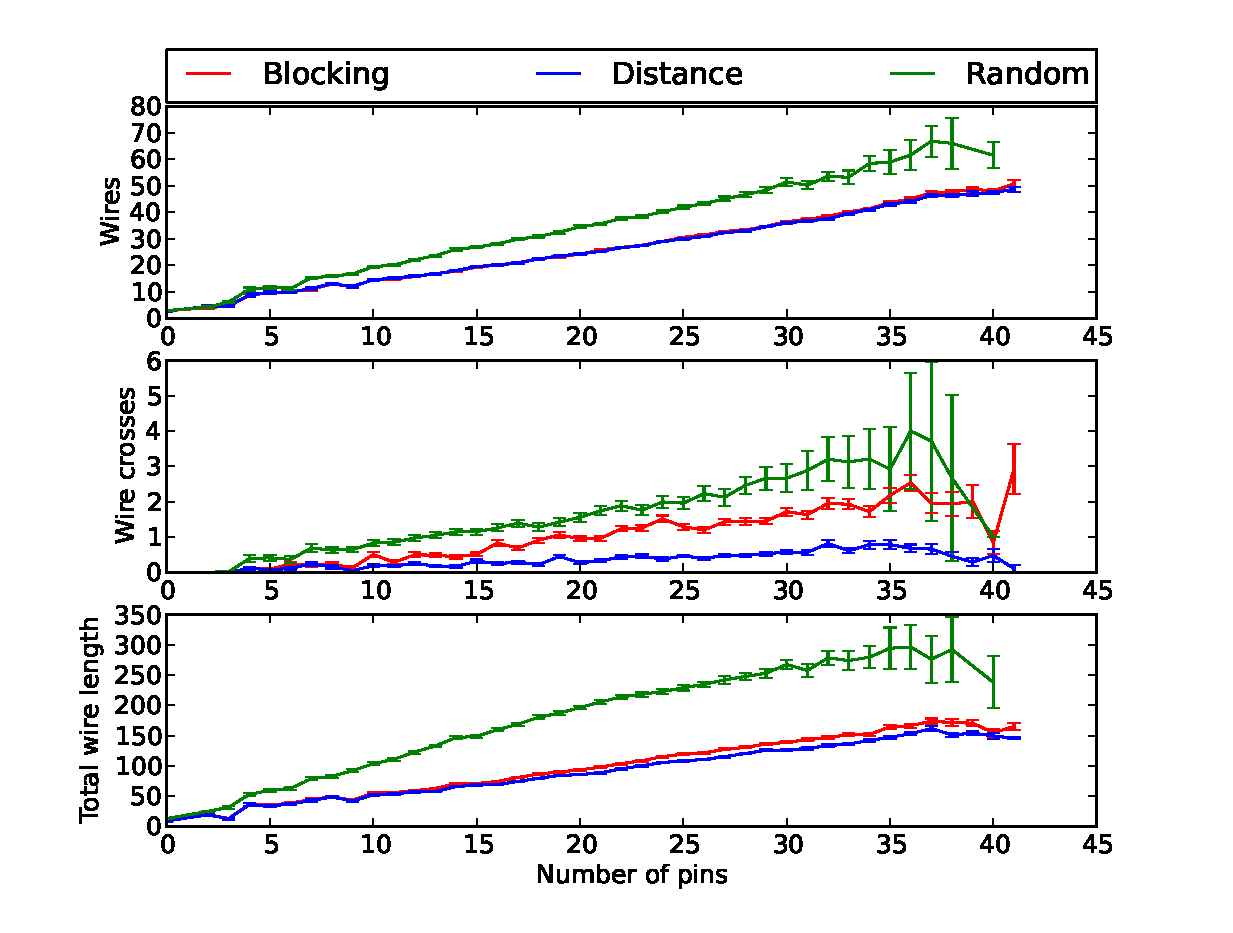
\includegraphics[width=\textwidth]{Images/placement_quality_trend_comparison.eps}
\caption[Placement method layout quality trend comparison]{Placement method
layout quality trend comparison.}
\label{fig:placement_quality_trend}
\end{center}
\end{figure}

\begin{figure}
\begin{center}
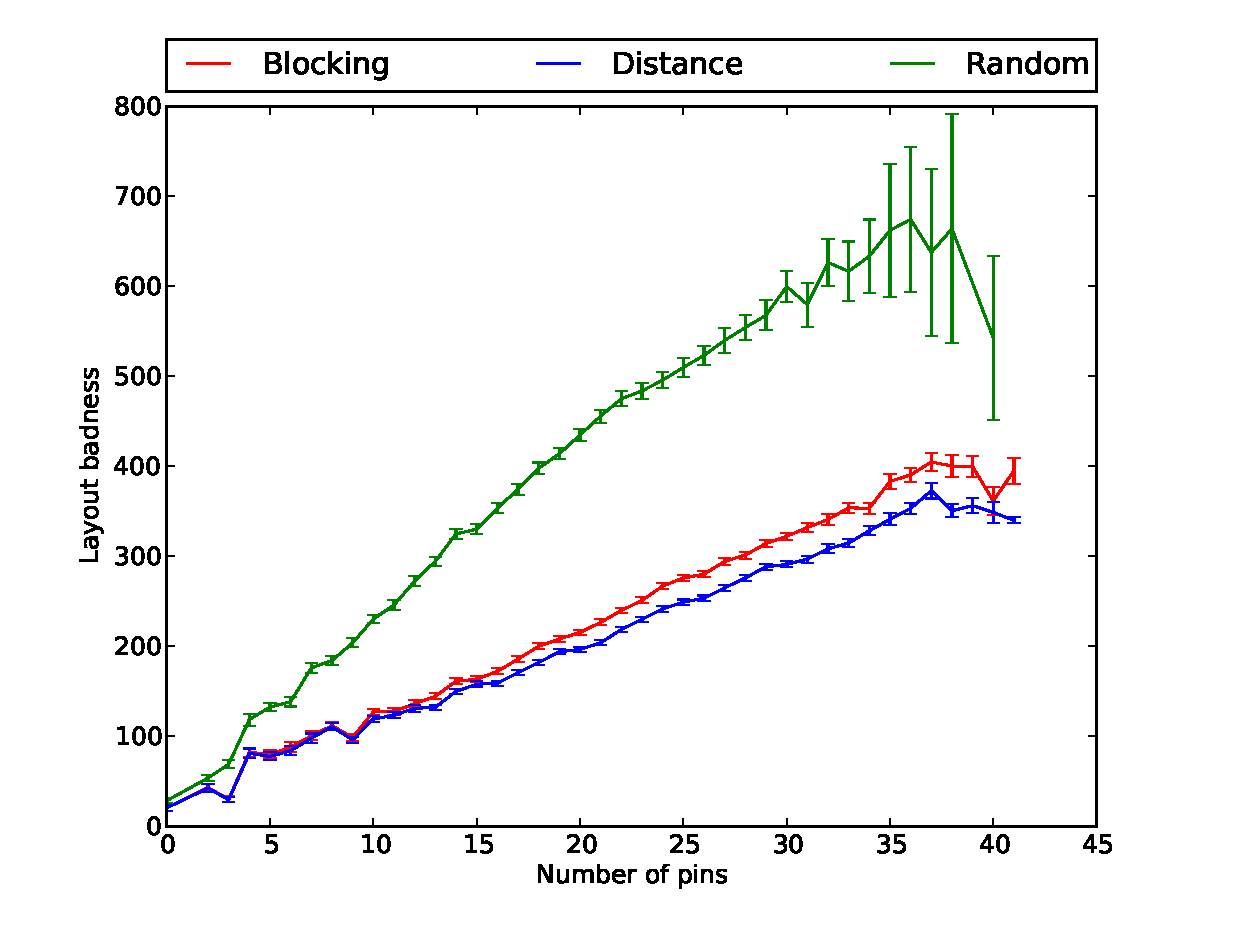
\includegraphics[width=\textwidth]{Images/placement_badness_trend_comparison.eps}
\caption[Placement method layout badness trend comparison]{Placement method
layout badness trend comparison.}
\label{fig:placement_badness_trend}
\end{center}
\end{figure}

\section{Comparing Wiring Methods}

\begin{figure}[H]
\begin{center}
\includegraphics[width=\textwidth]{Images/exemplar_all_pairs.png}
\caption[All pairs method exemplar]{Exemplar for the all pairs wiring method,
using blocking placement and $A*$ Search.}
\end{center}
\end{figure}

\begin{figure}[H]
\begin{center}
\includegraphics[width=\textwidth]{Images/exemplar_per_node_increasing.png}
\caption[Per-node (increasing) method exemplar]{Exemplar for the per-node
(increasing) wiring method, using blocking placement and $A*$ Search.}
\end{center}
\end{figure}

\begin{figure}[H]
\begin{center}
\includegraphics[width=\textwidth]{Images/exemplar_per_node_decreasing.png}
\caption[Per-node (decreasing) method exemplar]{Exemplar for the per-node
(decreasing) wiring method, using distance placement and $A*$ Search. We used
distance placement instead of blocking placement to generate this
exemplar because the combination of blocking placement with this wiring
method consistently failed on the schematic shown in Figure
\ref{fig:exemplar_schematic}.}
\end{center}
\end{figure}

\begin{figure}[H]
\begin{center}
\includegraphics[width=\textwidth]{Images/exemplar_per_pair_increasing.png}
\caption[Per-pair (increasing) method exemplar]{Exemplar for the per-pair
(increasing) wiring method, using blocking placement and $A*$ Search.}
\end{center}
\end{figure}

\begin{figure}[H]
\begin{center}
\includegraphics[width=\textwidth]{Images/exemplar_per_pair_decreasing.png}
\caption[Per-pair (decreasing) method exemplar]{Exemplar for the per-pair
(decreasing) wiring method, using blocking placement and $A*$ Search.}
\end{center}
\end{figure}

\begin{figure}[H]
\begin{center}
\includegraphics[width=\textwidth]{Images/exemplar_straight_wiring.png}
\caption[Straight wiring method exemplar]{
Exemplar for the straight wiring method, using blocking placement.}
\end{center}
\end{figure}

\begin{figure}[H]
\begin{center}
\includegraphics[width=15cm]{Images/wiring_success_comparison.eps}
\caption[Wiring method success rate comparison]{Wiring method success rate
comparison.}
\label{fig:wiring_success}
\end{center}
\end{figure}

\begin{table}[H]
\begin{center}
\begin{singlespace}
\begin{tabular}{|c||c|c|c|c|c|c|c|c|c|c|c|}
\hline
 & \multicolumn{11}{|c|}{Number of times succeeded out of $10$} \\
\hline
 & 0 & 1 & 2 & 3 & 4 & 5 & 6 & 7 & 8 & 9 & 10 \\
\hline\hline
All & $458$ & $114$ & $111$ & $112$ & $127$ & $145$ & $177$ & $139$ & $172$ & $227$ & $2643$ \\
 & $0.10$ & $0.03$ & $0.03$ & $0.03$ & $0.03$ & $0.03$ & $0.04$ & $0.03$ & $0.04$ & $0.05$ & $0.60$ \\
\hline
 Node I & $154$ & $50$ & $55$ & $62$ & $85$ & $71$ & $106$ & $141$ & $156$ & $217$ & $3328$ \\
  & $0.03$ & $0.01$ & $0.01$ & $0.01$ & $0.02$ & $0.02$ & $0.02$ & $0.03$ & $0.04$ & $0.05$ & $0.75$ \\
\hline
  Node D & $195$ & $50$ & $58$ & $66$ & $104$ & $83$ & $125$ & $176$ & $162$ & $268$ & $3138$ \\
   & $0.04$ & $0.01$ & $0.01$ & $0.01$ & $0.02$ & $0.02$ & $0.03$ & $0.04$ & $0.04$ & $0.06$ & $0.71$ \\
\hline
   Pair I & $177$ & $40$ & $59$ & $54$ & $91$ & $92$ & $100$ & $118$ & $132$ & $212$ & $3350$ \\
    & $0.04$ & $0.01$ & $0.01$ & $0.01$ & $0.02$ & $0.02$ & $0.02$ & $0.03$ & $0.03$ & $0.05$ & $0.76$ \\
\hline
    Pair D & $162$ & $38$ & $51$ & $57$ & $72$ & $85$ & $109$ & $106$ & $144$ & $203$ & $3398$ \\
     & $0.04$ & $0.01$ & $0.01$ & $0.01$ & $0.02$ & $0.02$ & $0.02$ & $0.02$ & $0.03$ & $0.05$ & $0.77$ \\
\hline
     Straight & $0$ & $0$ & $0$ & $0$ & $0$ & $0$ & $0$ & $0$ & $0$ & $0$ & $4425$ \\
      & $0.00$ & $0.00$ & $0.00$ & $0.00$ & $0.00$ & $0.00$ & $0.00$ & $0.00$ & $0.00$ & $0.00$ & $1.00$ \\
\hline
\end{tabular}
\end{singlespace}
\end{center}
\caption[Wiring method success rate comparison]{Wiring method success rate
comparison.}
\label{tb:wiring_success}
\end{table}

\begin{figure}[H]
\centering
\subfigure[All pairs]{
\includegraphics[width=8cm]{Images/wiring_all_success_trend.eps}}
\subfigure[Per-node]{
\includegraphics[width=8cm]{Images/wiring_node_success_trend.eps}}
\subfigure[Per-pair]{
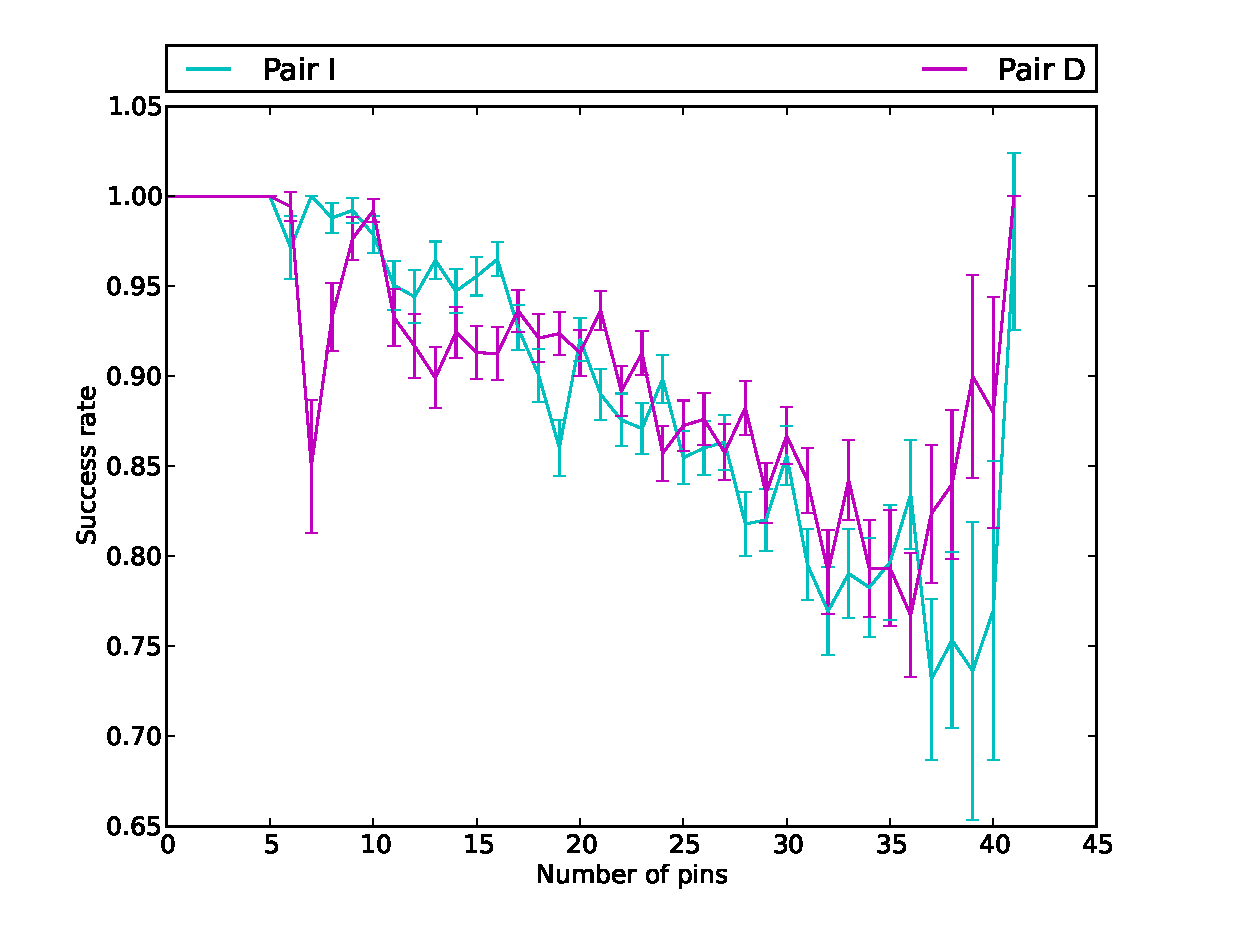
\includegraphics[width=8cm]{Images/wiring_pair_success_trend.eps}}
\caption[Wiring method success rate trend comparison]{Wiring method success rate
trend comparison.}
\label{fig:wiring_success_trend}
\end{figure}

\begin{figure}
\begin{center}
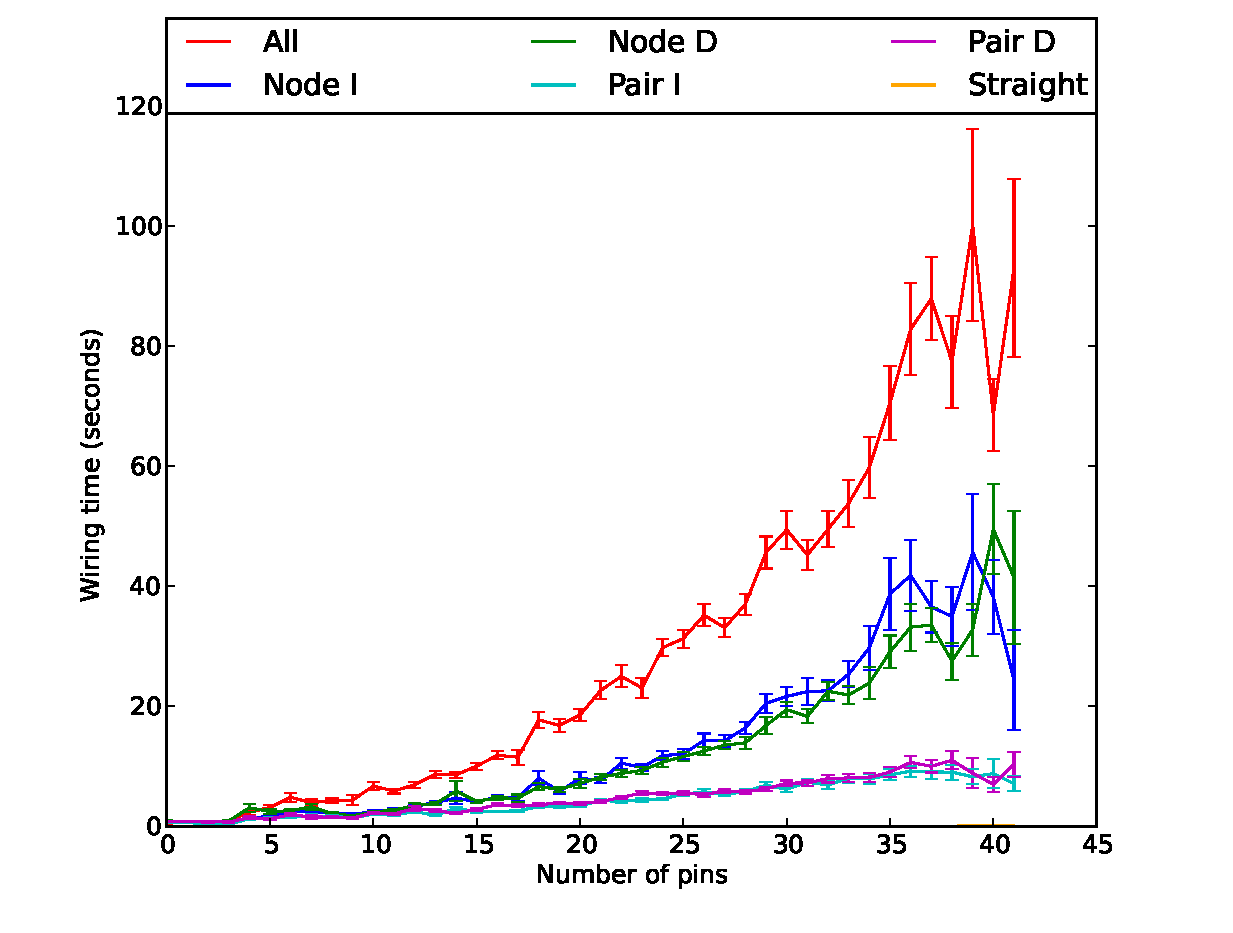
\includegraphics[width=\textwidth]{Images/wiring_time_trend_comparison.eps}
\caption[Wiring method wiring time trend comparison]{Wiring method wiring time
trend comparison for successful runs. Note that the line for Straight wiring is
not visible because it is so close to $0$ for all values of circuit complexity.}
\label{fig:wiring_time_trend}
\end{center}
\end{figure}

\begin{figure}
\begin{center}
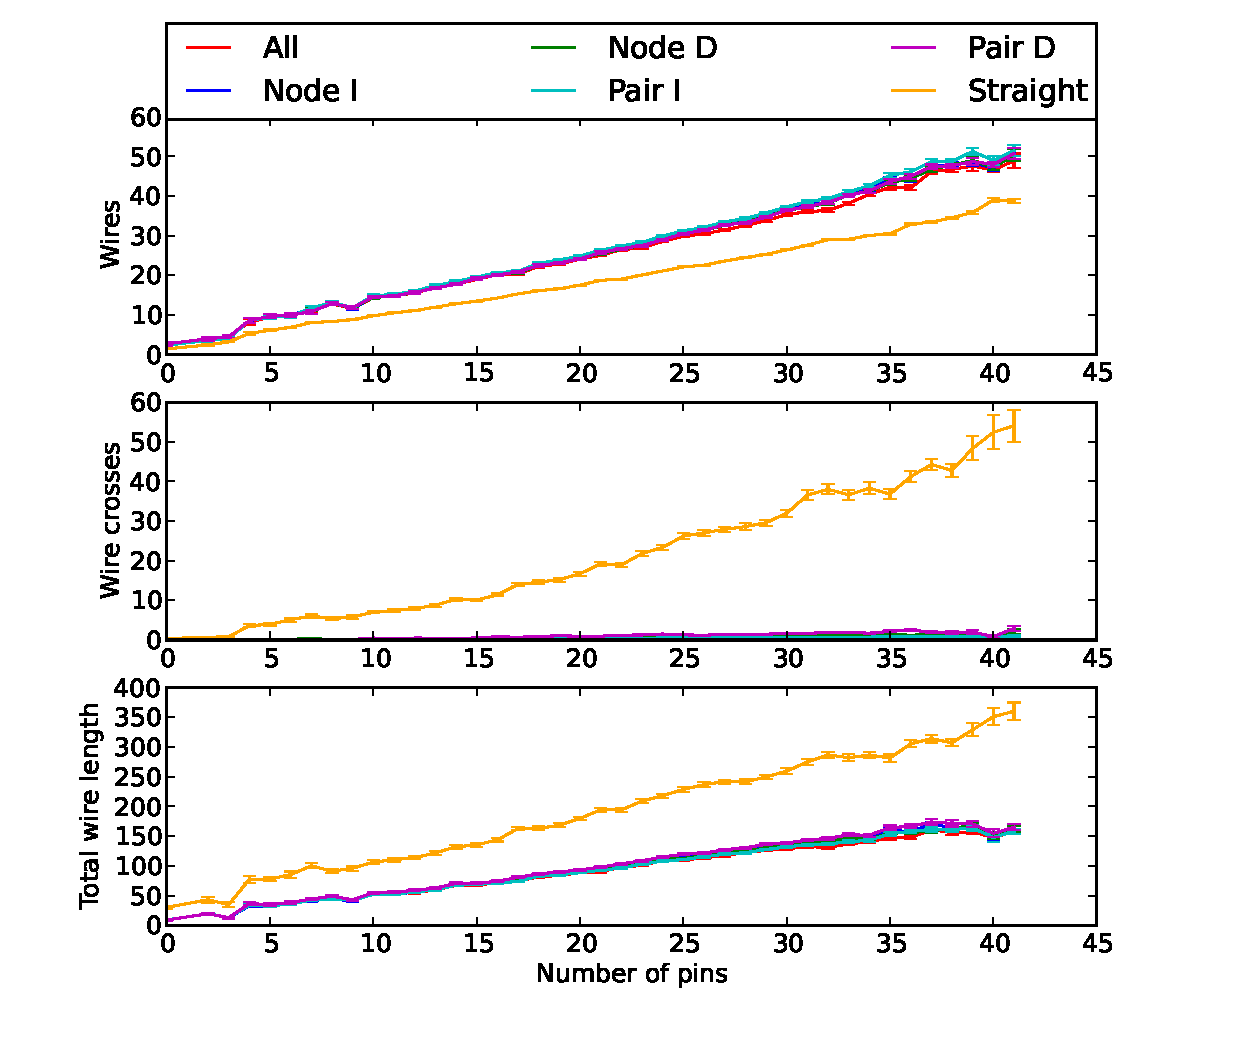
\includegraphics[width=\textwidth]{Images/wiring_quality_trend_comparison.eps}
\caption[Wiring method layout quality trend comparison]{Wiring method layout
quality trend comparison.}
\label{fig:wiring_quality_trend}
\end{center}
\end{figure}

\begin{figure}
\begin{center}
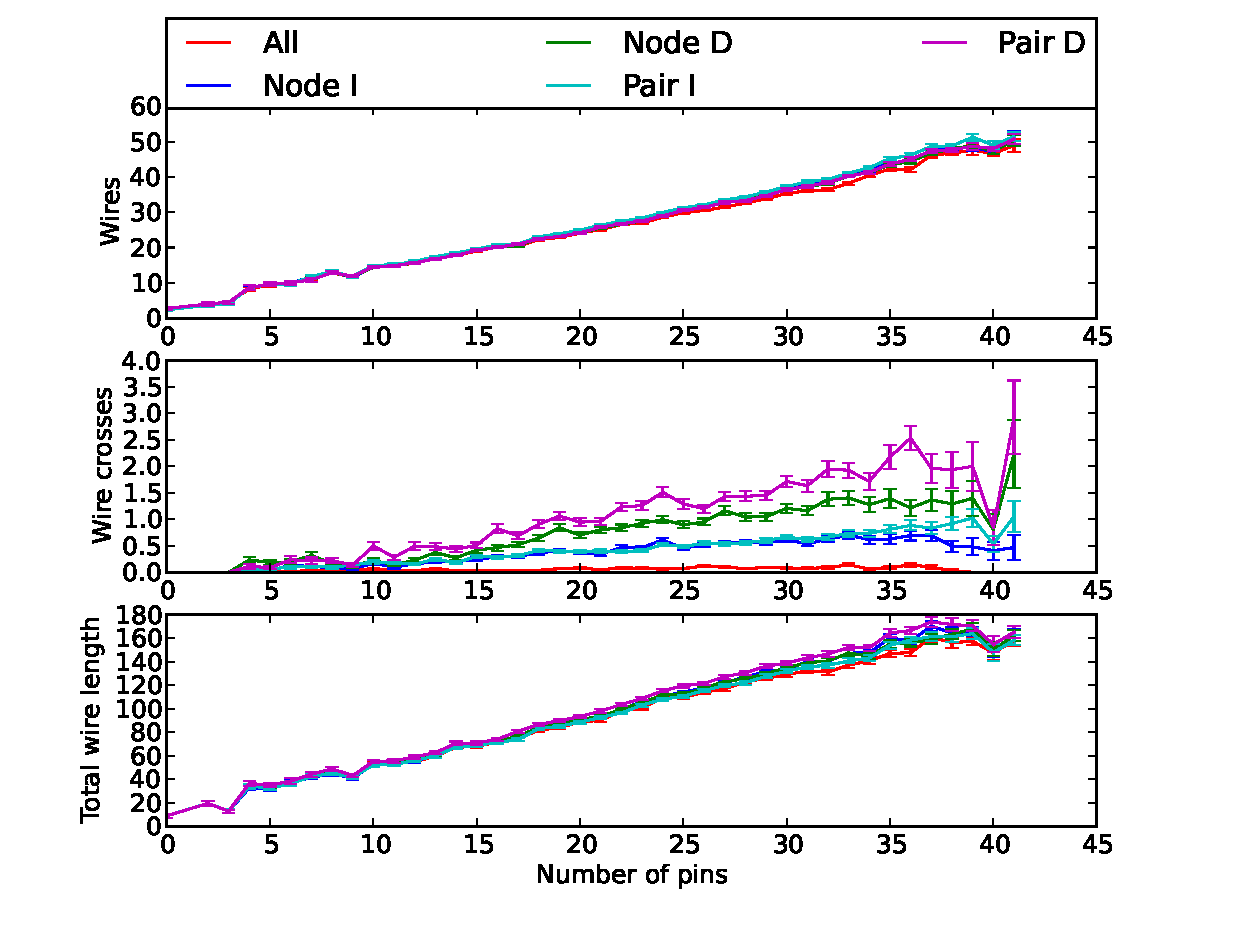
\includegraphics[width=\textwidth]{Images/wiring_quality_trend_comparison_no_straight.eps}
\caption[Wiring method layout quality trend comparison (without Straight wiring)]
{Wiring method layout quality trend comparison, not including the Straight
wiring method.}
\label{fig:wiring_quality_trend_no_straight}
\end{center}
\end{figure}

\begin{figure}
\begin{center}
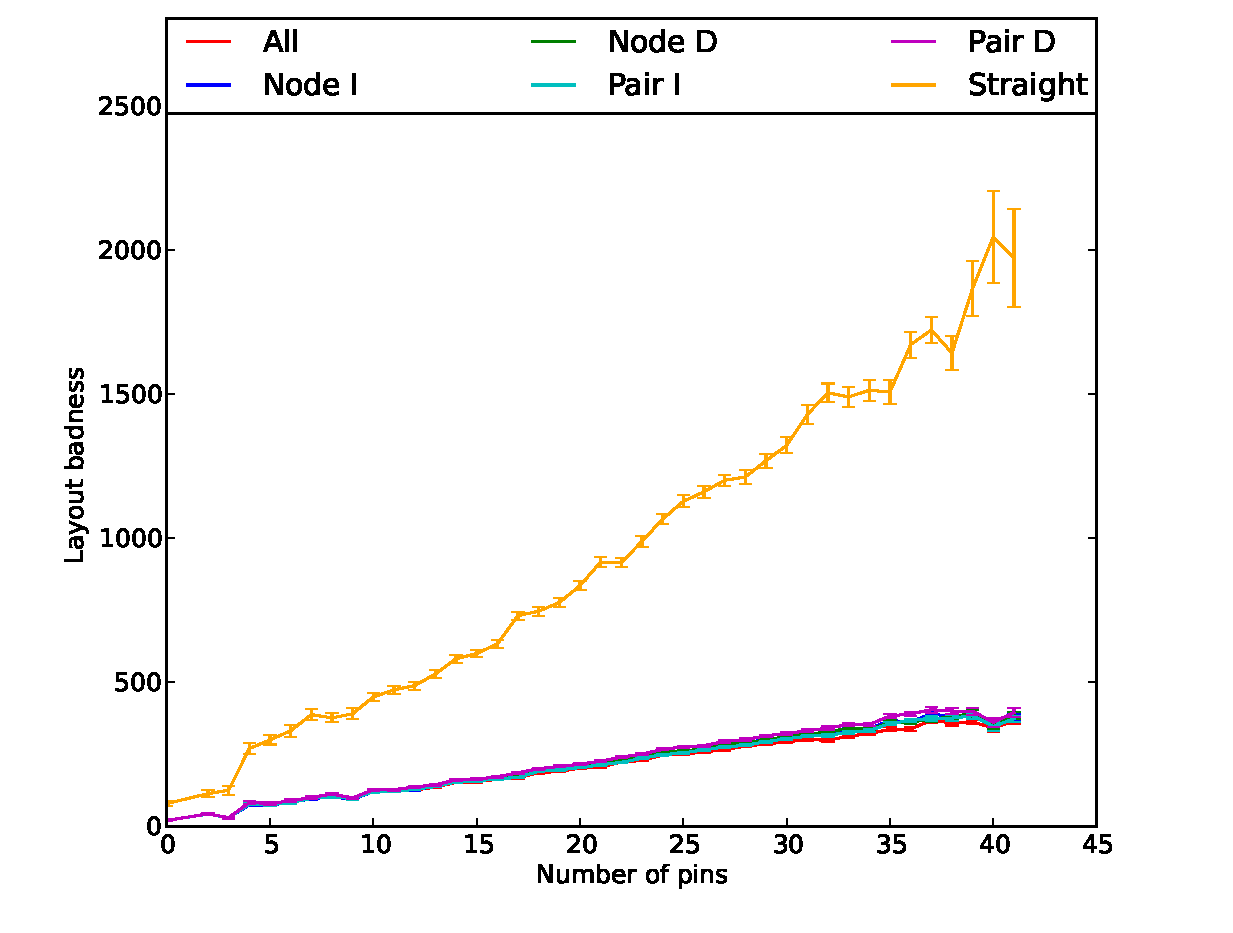
\includegraphics[width=\textwidth]{Images/wiring_badness_trend_comparison.eps}
\caption[Wiring method layout badness trend comparison]{Wiring method layout
badness trend comparison.}
\label{fig:wiring_badness_trend}
\end{center}
\end{figure}

\section{Comparing Search Methods}

\begin{figure}[H]
\begin{center}
\includegraphics[width=\textwidth]{Images/exemplar_per_pair_decreasing.png}
\caption[$A*$ Search exemplar]{Exemplar for $A*$ Search, using blocking
placement and per-pair (decreasing) wiring.}
\end{center}
\end{figure}

\begin{figure}[H]
\begin{center}
\includegraphics[width=\textwidth]{Images/exemplar_best_first.png}
\caption[Best First Search exemplar]{Exemplar for Best First Search, using
blocking placement and per-pair (decreasing) wiring.}
\end{center}
\end{figure}

\begin{figure}[H]
\begin{center}
\includegraphics[width=\textwidth]{Images/search_success_comparison.eps}
\caption[Search method success rate comparison]{Search method success rate
comparison.}
\label{fig:search_success}
\end{center}
\end{figure}

\begin{table}[H]
\begin{center}
\begin{singlespace}
\begin{tabular}{|c||c|c|c|c|c|c|c|c|c|c|c|}
\hline
 & \multicolumn{11}{|c|}{Number of times succeeded out of $10$} \\
\hline
 & 0 & 1 & 2 & 3 & 4 & 5 & 6 & 7 & 8 & 9 & 10 \\
\hline\hline
$A*$ & $162$ & $38$ & $51$ & $57$ & $72$ & $85$ & $109$ & $106$ & $144$ & $203$ & $3398$ \\
 & $0.04$ & $0.01$ & $0.01$ & $0.01$ & $0.02$ & $0.02$ & $0.02$ & $0.02$ & $0.03$ & $0.05$ & $0.77$ \\
\hline
 Best First & $6$ & $5$ & $2$ & $1$ & $13$ & $10$ & $29$ & $45$ & $84$ & $245$ & $3985$ \\
  & $0.00$ & $0.00$ & $0.00$ & $0.00$ & $0.00$ & $0.00$ & $0.01$ & $0.01$ & $0.02$ & $0.06$ & $0.90$ \\
\hline
\end{tabular}
\end{singlespace}
\end{center}
\caption[Search method success rate comparison]{Search method success rate
comparison.}
\label{tb:search_success}
\end{table}

\begin{figure}
\begin{center}
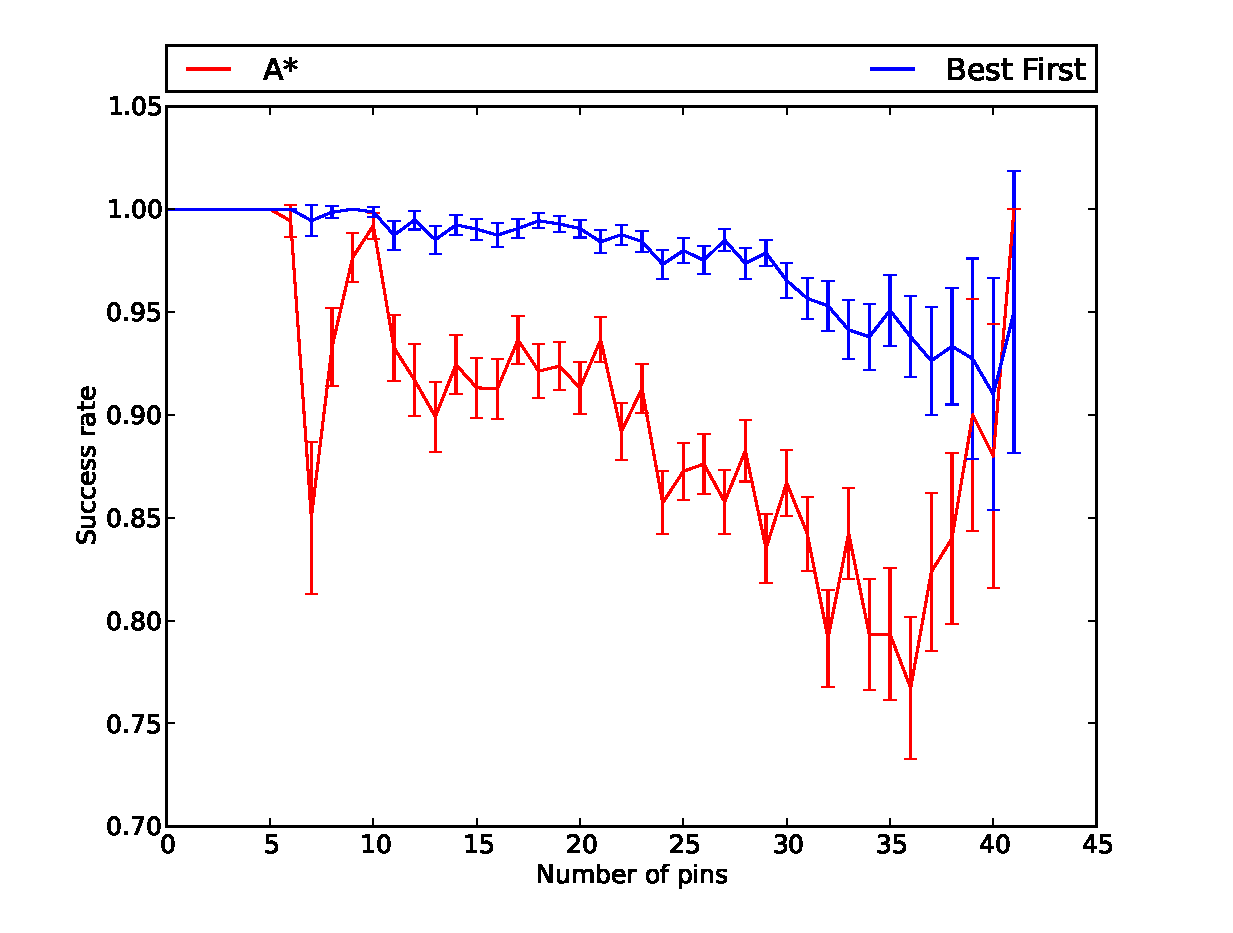
\includegraphics[width=\textwidth]{Images/search_success_trend_comparison.eps}
\caption[Search method success rate trend comparison]{Search method success rate
trend comparison.}
\label{fig:search_success_trend}
\end{center}
\end{figure}

\begin{figure}
\begin{center}
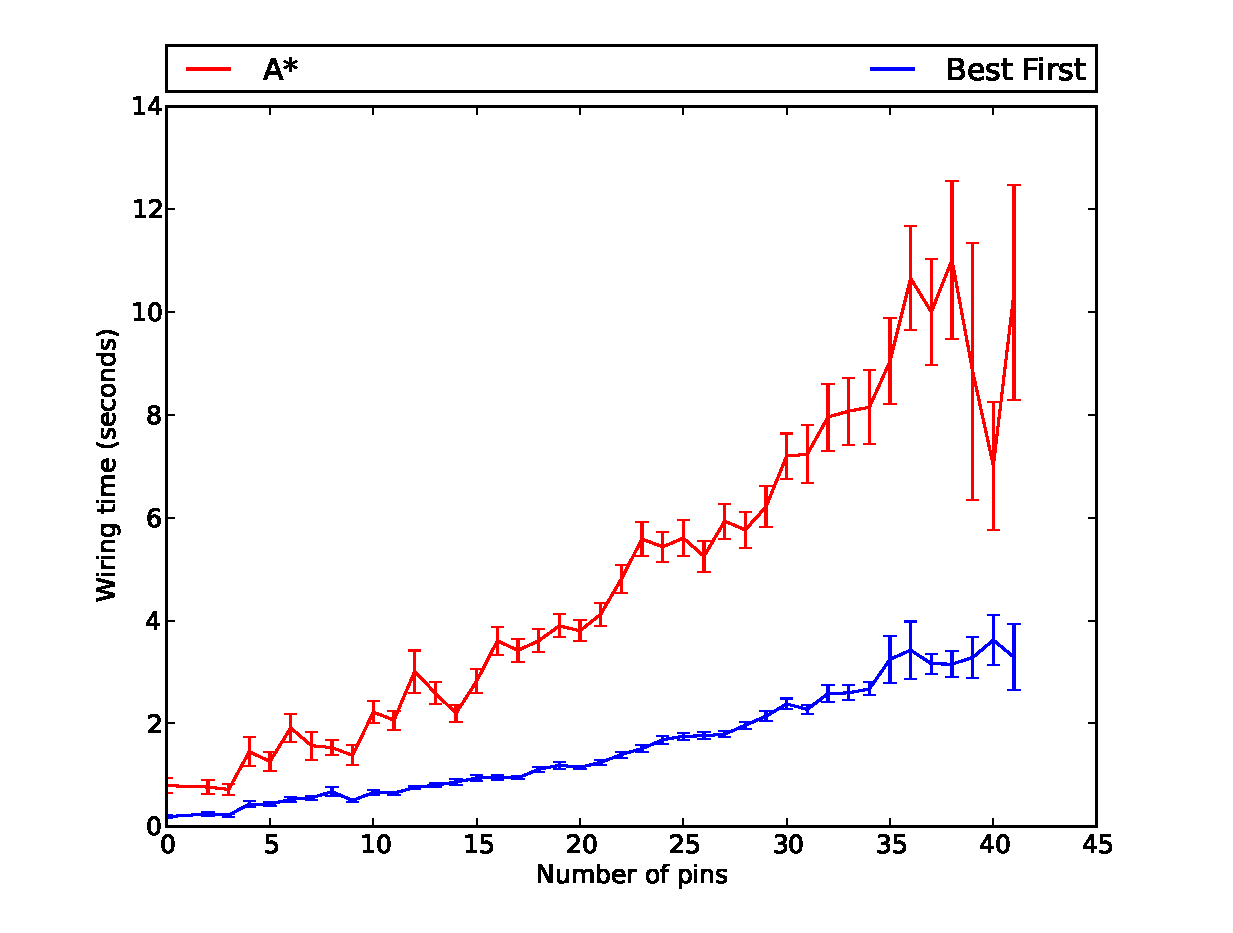
\includegraphics[width=\textwidth]{Images/search_time_trend_comparison.eps}
\caption[Search method wiring time trend comparison]{Search method wiring time
trend comparison for successful runs.}
\label{fig:search_time_trend}
\end{center}
\end{figure}

\begin{figure}
\begin{center}
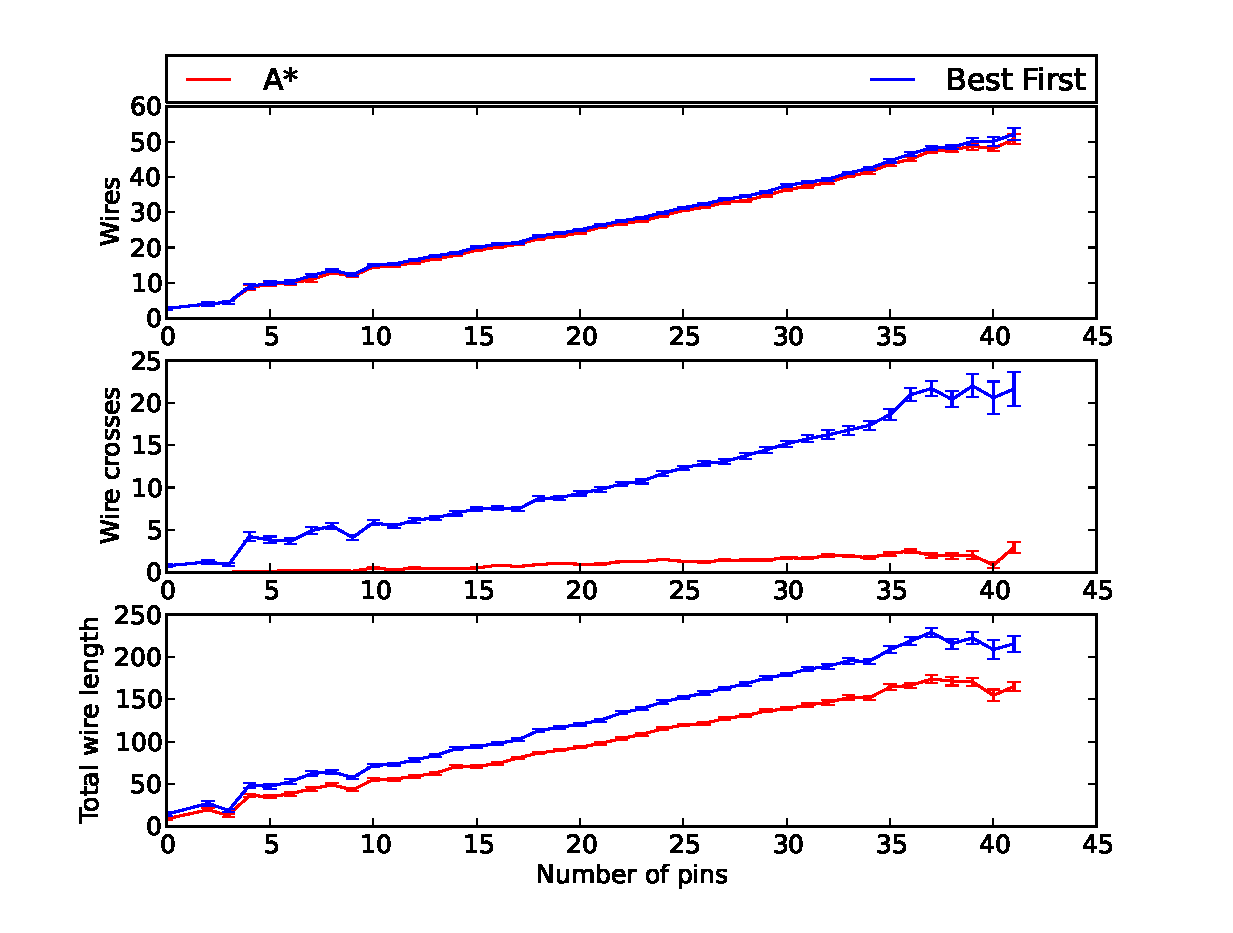
\includegraphics[width=\textwidth]{Images/search_quality_trend_comparison.eps}
\caption[Search method layout quality trend comparison]{Search method layout
quality trend comparison.}
\label{fig:search_quality_trend}
\end{center}
\end{figure}

\begin{figure}
\begin{center}
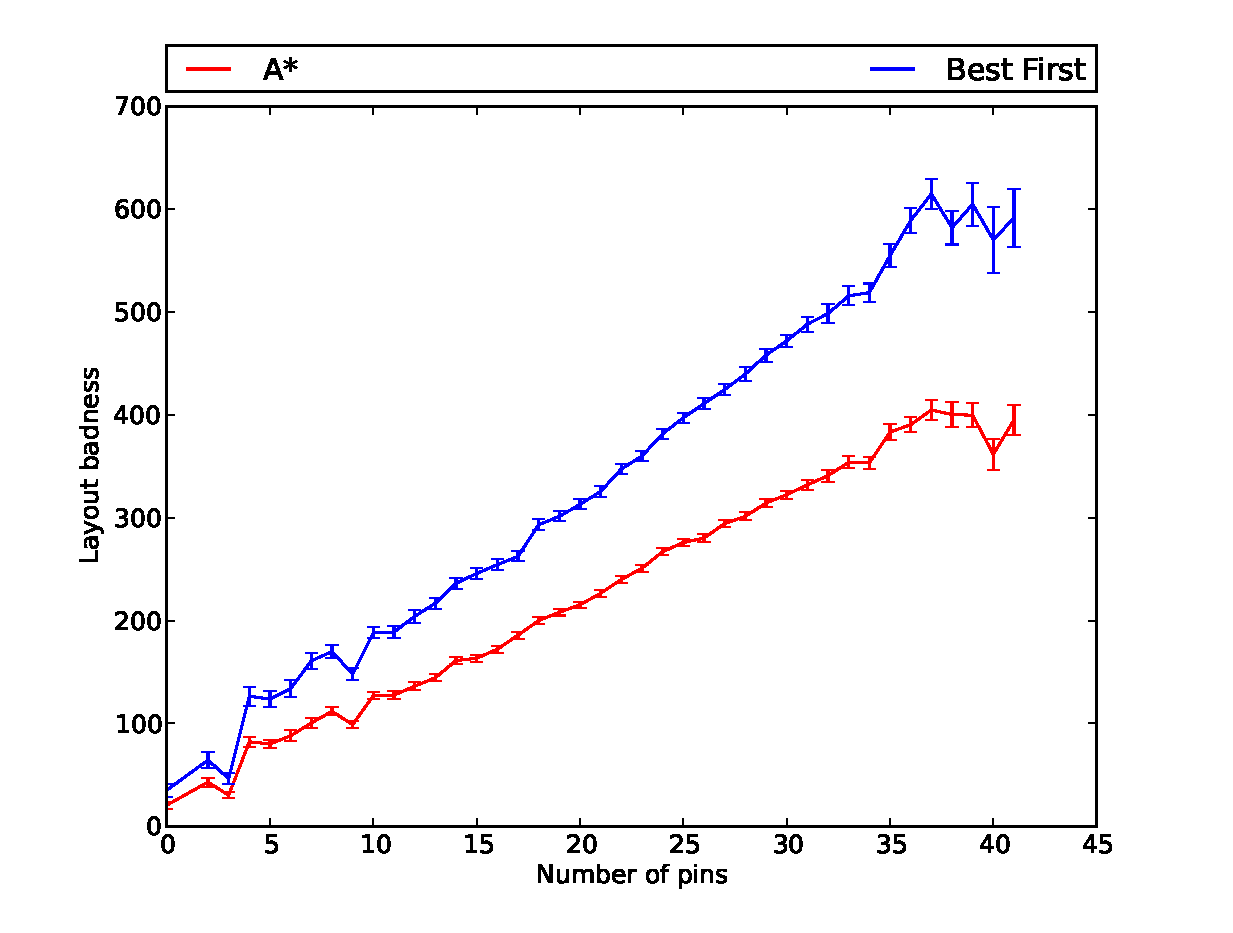
\includegraphics[width=\textwidth]{Images/search_badness_trend_comparison.eps}
\caption[Search method layout badness trend comparison]{Search method layout
badness trend comparison.}
\label{fig:search_badness_trend}
\end{center}
\end{figure}

\newpage\section{Combined Algorithm}
\label{sec:combined_algorithm}

Here we provide data for the combined algorithm presented in Section
\ref{sec:combined_alg}. To generate this data, we used a different dataset of
$4425$ schematics. As desired, the algorithm has a $100\%$ success rate.
Figure \ref{fig:final_num_trials} gives a breakdown of how the algorithm
succeeded. The first four columns correspond to success from one of the four
combinations of placement and wiring methods. The last 5 columns correspond to
layouts in which none of the four combinations was successful on all pairs of
locations and the algorithm had to connect a few pairs of locations by putting
down a straight wire bridging the locations. Figure
\ref{fig:final_time_trend} gives the average total time taken by the algorithm
as a function of circuit complexity. Finally, Figures
\ref{fig:final_quality_trend} and \ref{fig:final_badness_trend}
give statistics on the quality of the layouts produced by the combined algorithm
as a function of circuit complexity. Some of the plots in this section compare
the final algorithm to the completely random strategy
presented in Section \ref{sec:random_layout}.

\begin{figure}[H]
\begin{center}
\includegraphics[width=\textwidth]{Images/exemplar_combined_algorithm.png}
\caption[Combined algorithm exemplar]{Combined algorithm exemplar. Notice that
the top rail rows (the first and second row) are forced to be used as power and
ground nodes.}
\end{center}
\end{figure}

\begin{figure}
\begin{center}
\includegraphics[width=\textwidth]{Images/final_algorithm_num_trials.eps}
\caption[Combined algorithm success summary]{Combined algorithm success summary.}
\label{fig:final_num_trials}
\end{center}
\end{figure}

\begin{figure}
\begin{center}
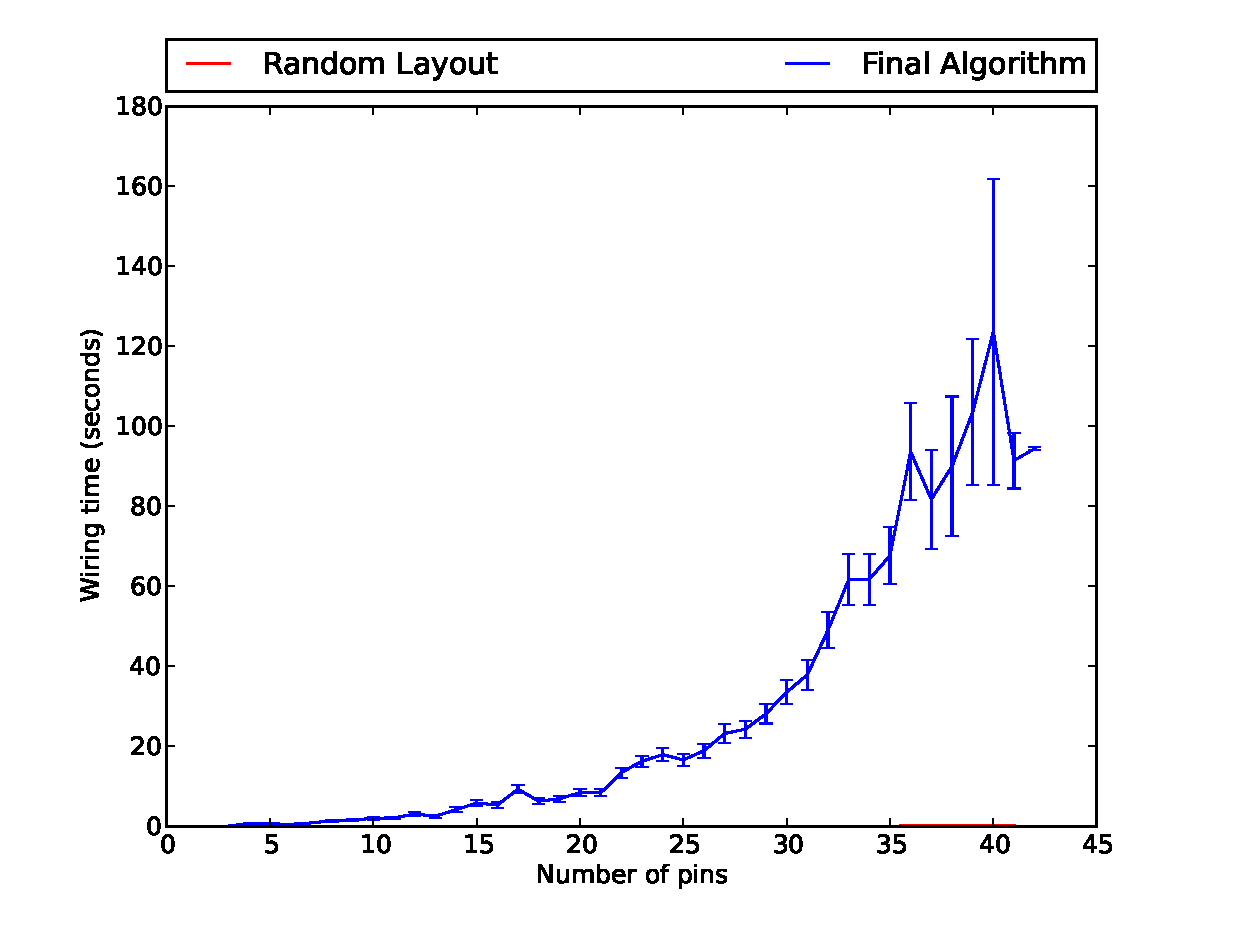
\includegraphics[width=\textwidth]{Images/final_algorithm_time_trend.eps}
\caption[Combined algorithm time trend]{Total CPU time trend comparison.
Note that the line for Random Layout is
not visible because it is so close to $0$ for all values of circuit complexity.}
\label{fig:final_time_trend}
\end{center}
\end{figure}

\begin{figure}
\begin{center}
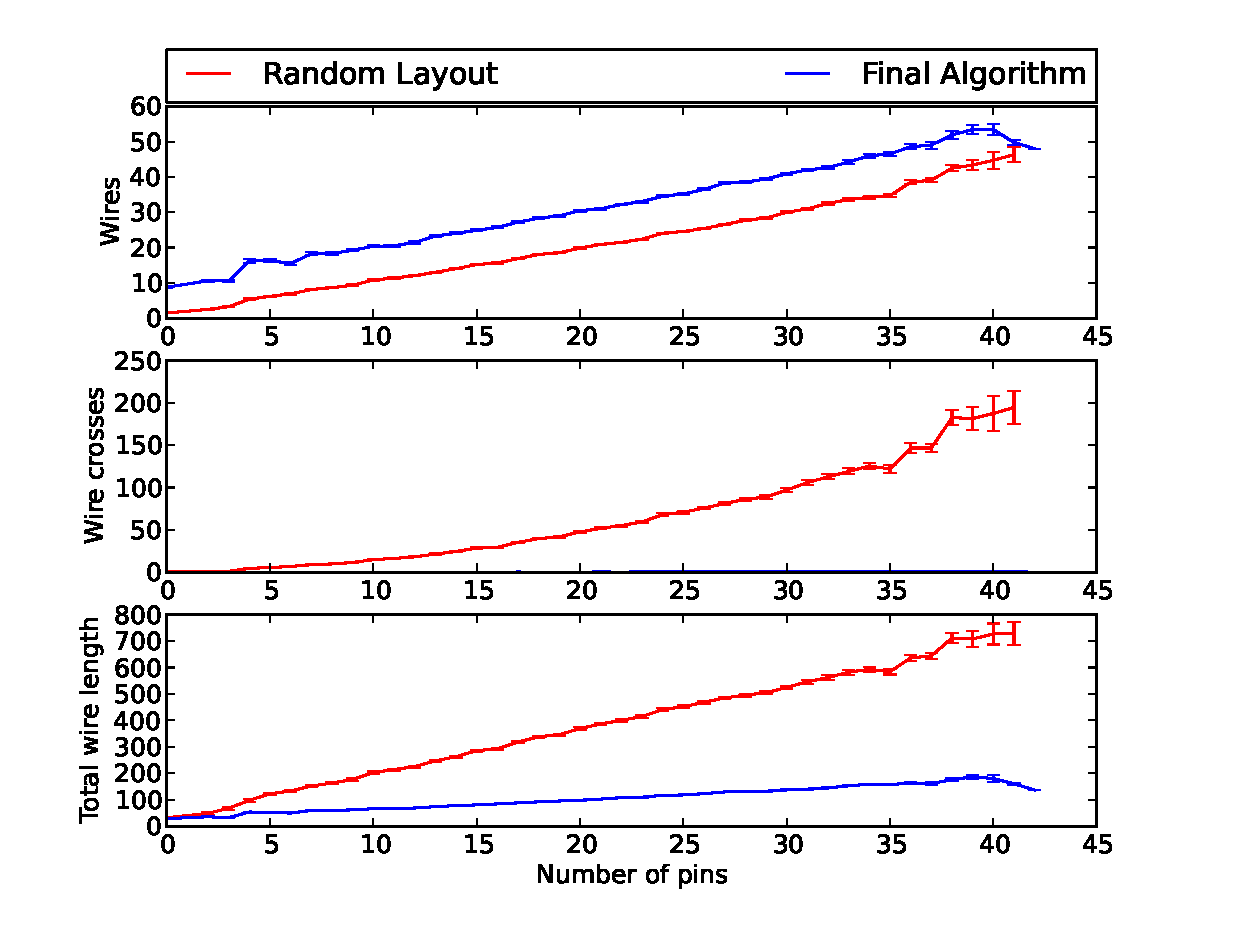
\includegraphics[width=\textwidth]{Images/final_algorithm_quality_trend.eps}
\caption[Combined algorithm layout quality trend]{Layout quality trend
comparison. Note that the line for number of wire crosses for the Final
Algorithm is not visible because it is so much closer to $0$ than the number
of wire crosses for Random Layout for all values of circuit complexity.}
\label{fig:final_quality_trend}
\end{center}
\end{figure}

\begin{figure}
\begin{center}
\includegraphics[width=\textwidth]{Images/final_algorithm_badness_trend.eps}
\caption[Combined algorithm layout badness trend]{Layout badness trend.}
\label{fig:final_badness_trend}
\end{center}
\end{figure}
